\documentclass[tikz,border=2pt]{standalone}
\usepackage{amsmath}
\usepackage{pgfplots}
\pgfplotsset{compat=1.18}

\begin{document}
% On a compact interval [a,b] a continuous function is uniformly continuous: one delta-window
% width (here 0.3) keeps the graph inside the same epsilon-band (height 0.6) wherever the
% window is placed, even where f = x^2/2 is at its steepest.
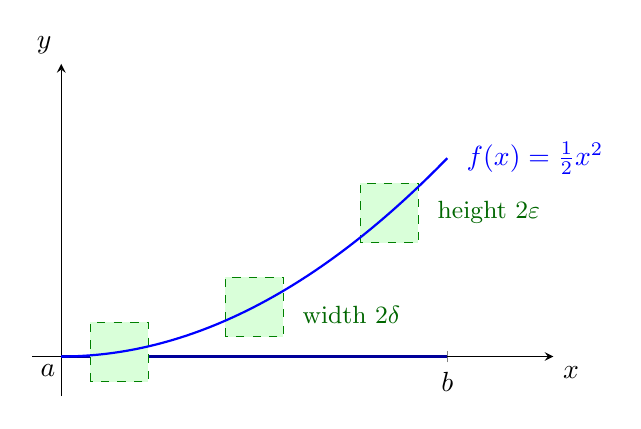
\begin{tikzpicture}
	\begin{axis}[
		axis lines=middle,
		xmin=-0.15, xmax=2.55,
		ymin=-0.4, ymax=2.95,
		xtick={2}, xticklabels={$b$}, ytick=\empty,
		xlabel={$x$}, ylabel={$y$},
		xlabel style={below right}, ylabel style={above left},
		samples=80, smooth, clip=false,
		width=8.2cm, height=5.8cm
		]
		\draw[very thick, blue!60!black] (axis cs:0,0) -- (axis cs:2,0);
		\fill[green!15] (axis cs:0.15,-0.255) rectangle (axis cs:0.45,0.345);
		\draw[green!50!black, dashed] (axis cs:0.15,-0.255) rectangle (axis cs:0.45,0.345);
		\fill[green!15] (axis cs:0.85,0.2) rectangle (axis cs:1.15,0.8);
		\draw[green!50!black, dashed] (axis cs:0.85,0.2) rectangle (axis cs:1.15,0.8);
		\fill[green!15] (axis cs:1.55,1.145) rectangle (axis cs:1.85,1.745);
		\draw[green!50!black, dashed] (axis cs:1.55,1.145) rectangle (axis cs:1.85,1.745);
		\addplot[thick, blue, domain=0:2] {x^2/2};
		\node[anchor=north east, inner sep=2pt] at (axis cs:0,-0.02) {$a$};
		\node[blue, anchor=west] at (axis cs:2.05,2.0) {$f(x)=\tfrac12x^2$};
		\node[green!40!black, anchor=west, font=\small] at (axis cs:1.2,0.42) {width $2\delta$};
		\node[green!40!black, anchor=west, font=\small] at (axis cs:1.9,1.45) {height $2\varepsilon$};
	\end{axis}
\end{tikzpicture}
\end{document}
